

The \emph{expectation maximization} algorithm is an iterative method to find maximum likelihood or maximum a posteriori estimates of parameters in statistical models, where the model depends on hidden variables. The main idea is to set a lower bound to the marginal likelihood, then using an iterative method to increase this lower bound, and the marginal likelihood with it.

\subsection{General case}

Consider we have only two variables, one visible \(V\) and one hidden \(H\). Consider also the Kullback-Leibler divergence between a `variational' distribution \(Q(h\mid v)\) (where variational means that this distribution is the object of an optimization problem) and a parametric one \(P(h \mid v, \theta)\).
\[
  \begin{aligned}
    KL(Q(h\mid v) \mid P(h \mid v, \theta)) &= \E{Q}{\log{Q(h \mid v)} - \log{P(h \mid v, \theta)}} \\
    &= \E{Q}{\log{Q(h \mid v)}} - \E{Q}{\log{P(h,v \mid \theta)}} + \E{Q}{\log{P(v \mid \theta)}}\\
    &= \E{Q}{\log{Q(h \mid v)}} - \E{Q}{\log{P(h,v \mid \theta)}} + \log{P(v \mid \theta)} \geq 0
  \end{aligned}
\]
We got then a lower bound for \(\log P(v \mid \theta)\)
\[
  \log{P(v \mid \theta)}\geq \underbrace{-\E{Q}{\log{Q(h \mid v)}}}_{\text{Entropy}} + \underbrace{\E{Q}{\log{P(h,v \mid \theta)}}}_{\text{Energy}}\footnote{Energy and Entropy  terms come from a statistical physics terminology}
\]
Assume a set of observations, \(\V = \{x_{1}, \dots, x_{N}\}\) where each \(x_{n} = (v_{n}, h_{n})\) where \(v_{n}\) is the visible o the visible variables and \(h_{n}\) denotes a state of the hidden ones, that is, it is not fixed for each data-point. Then, has the variables of the observations are i.i.d we got that
\[
    \log{P(v_{1},\dots,v_{N} \mid \theta)} = \sum_{n=1}^{N}\log{P(v_{n} \mid \theta)} \geq \sum_{n = 1}^{N} -\E{Q}{\log{Q(h_{n} \mid v_{n})}} + \E{Q}{\log{P(h_{n},v_{n} \mid \theta)}}
\]
And we know equality holds if and only if \(Q(h_{n} \mid v_{n}) = P(h_{n} \mid v_{n} , \theta) \ \forall n=1, \dots, N\).

This suggest the following iterative procedure to optimize the parameter \(\theta\) consisted in two steps.
\begin{itemize}
  \item \textbf{E-step}. For a fixed \(\theta\), find the distributions that maximize the above bound, i.e, choose \(Q(h_{n} \mid v_{n}) = P(h_{n} \mid v_{n} , \theta)\).
  \item \textbf{M-step}. For a fixed distribution \(Q\), find the parameter \(\theta\) that maximizes the bound. Since \(Q\) does not depend on the parameter, this is equivalent to maximize the energy term.
\end{itemize}

\begin{exampleth}
  Consider a single variable \(V\) with \(Dom(V) = \mathbb{R}\) and a single hidden variable \(H\) with \(dom(H) = \{1,2\}\). Consider the model
  \[
    P(v \mid h, \theta) = \frac{1}{\sqrt{\pi}}e^{-(v - \theta h)^{2}}
  \]
  and \(P(H = 1) = P(H = 2) = 0.5\). Suppose an observation \(v = 2.75\) we want to optimize the parameter \(\theta\) in the marginal
  \[
    P(V = 2.75 \mid \theta) = \int_{h} P(V = 2.75 \mid h, \theta) P(h) = \frac{1}{2\sqrt{\pi}}\big( e^{-(2.75 - \theta)^{2}} + e^{-(2.75 - 2\theta)^{2}} \big)
  \]

  Then using a distribution \(Q(h \mid v)\), the lower bound given to the log likelihood is
  \[
    \log{P(v \mid \theta)} \geq -Q(1 \mid 2.75)\log{Q(1 \mid 2.75)} - Q(2 \mid 2.75)\log{Q(2 \mid 2.75)} - \E{Q}{(v - \theta h)^{2}}\ + \text{const.}
  \]
  The M-step can be done analytically, noticing that due to the negative sign we want to minimize \(\E{Q}{(v - \theta h)^{2}}\)
  \[
    \frac{d}{d\theta}\E{Q}{(v - \theta h)^{2}} = \E{Q}{ 2 v h + 2\theta h^{2} } = 2v\E{Q}{h} + 2\theta \E{Q}{h^{2}} = 0 \iff \theta = \frac{v\E{Q}{h}}{\E{Q}{h^{2}}}
  \]
  \[
     \frac{d^{2}}{d^{2}\theta}\E{Q}{(v - \theta h)^{2}} = 2\E{Q}{h^{2}} \geq 0
  \]

  so the new parameter optimal parameter is
  \[
    \theta_{new} = v \frac{\E{Q}{H}}{\E{Q}{H^{2}}}
  \]

  The E-step would set \(Q_{new}(h \mid v) = P(h \mid v , \theta)\), in this case
  \[
    Q_{new}(h) = \frac{P(V = 2.75 \mid h, \theta)P(H = 2)}{P(V = 2.75)} = \frac{e^{-(2.75-h\theta)}}{ e^{-(2.75-\theta)} + e^{-(2.75-2\theta)}  }
  \]
\end{exampleth}

 \begin{algorithm}[t]
  \SetAlgoLined
  \KwData{A distribution \(P(x \mid \theta)\) and a dataset \(\V\). Where \(X\) splits in visible variables \(V\) and hidden variables \(H\)}
  \KwResult{Parameter \(\theta\) that maximizes the likelihood}
  \While{Convergence stop criteria}{
    \For{\(n \in 1,\dots,N\)}{
      \(Q(h \mid v_{n}) = P(h \mid v_{n}, \theta)\)\;
    }
    \(\theta = \argmax_{\theta}\sum_{n=1}^{N}\E{Q(h \mid v_{n})}{\log{P(h, v_{n} \mid \theta)}}\)\;
  }
  \KwRet{\(\theta\)}\;
  \caption{Expectation Maximization Algorithm}
  \label{alg:em}
\end{algorithm}

\subsection{EM increases the marginal likelihood}

It is clear that the EM algorithm does increase the lower bound in each iteration but we would like it to increase not only the bound but also the marginal likelihood. We will be using a single data point as it easy holds by summation when using the full dataset.

Let \(\theta^{new}\) be the value of the parameter after one iteration, we assume that \(Q\) is set to
\[
  Q(h \mid v) = P(h \mid v, \theta)
\]
So the lower bound in terms of \(\theta\) and \(\theta^{new}\) is
\[
  LB(\theta^{new} \mid \theta) =  \underbrace{-\E{P(h \mid v, \theta)}{\log{P(h \mid v, \theta)}}}_{\text{Entropy}} + \underbrace{\E{P(h \mid v, \theta)}{\log{P(h,v \mid \theta^{new})}}}_{\text{Energy}}
\]

From the definition of the Kullback-Leibler we get that
\[
  \log{P(v \mid \theta^{new})} = LB(\theta^{new}\mid \theta) + \KL{P(h \mid v, \theta)}{P(h \mid v, \theta^{new})}
\]
We could use \(\theta\) in the above formula getting
\[
  \log{P(v \mid \theta)} = LB(\theta \mid \theta) + \KL{P(h \mid v, \theta)}{P(h \mid v, \theta)} = LB(\theta \mid \theta)
\]
So we can compute the difference between the log likelihood between two consecutive iterations as
\[
  \log{P(v \mid \theta^{new})} - \log{P(v \mid \theta)} = LB(\theta^{new}\mid \theta) - LB(\theta \mid \theta) +  \KL{P(h \mid v, \theta)}{P(h \mid v, \theta^{new})}
\]

Where we know the last term is always positive, about the difference of bounds, the M-step ensures the new parameter makes the lower bound higher or equal to the current one, so that difference is also positive.
\[
   \log{P(v \mid \theta^{new})} - \log{P(v \mid \theta)} \geq 0
\]

\subsection{Bayesian Networks case}

As we did before let \(\X = (\V, \mathcal{H}) = \{X_{1}, \dots , X_{M}\}\) be the set of variables partitioned in visible and hidden. Let \(\mathcal{D} = \{(v^{1},h^{1}),\dots,(v^{N},h^{N})\}\) be the set of observations.

As we are not using a single variable anymore, the variational distribution is now over the set of hidden variables conditioned on the visible \(Q(\mathcal{H} \mid \V)\). As the E-step is the same as in the general case, we are focusing on the M-step, where \(Q_{old}\) is fixed.

The \emph{energy term} in a Bayesian Network is
\[
  \sum_{n=1}^{N} \E{Q_{old}(h^{n} \mid v^{n})}{ \log{P(x^{n} \mid \theta)} } = \sum_{n = 1}^{N}\sum_{i = 0}^{M} \E{Q_{old}(h^{n} \mid v^{n})}{\log{P( x_{i}^{n} \mid pa(x_{i}^{n}), \theta)}}
\]

It is useful to use the following notation that defines a conditional distribution of the hidden variable when the visible one equals \(v^{n}\).
\[
  Q^{n}(x) = Q^{n}(v,h) = Q_{old}(h^{n} \mid v^{n}) \mathbb{I}(v = v^{n})
\]
We can define the mixture distribution
\[
  Q(x) = \frac{1}{N}\sum_{n = 1}^{N}Q^{n}(x)
\]
Then we have that
\[
  \begin{aligned}
    \E{Q(x)}{\log{P(x \mid \theta)}} &= \int_{x}Q(x)\log{P(x \mid \theta)} =  \int_{x} \frac{1}{N}\sum_{n=1}^{N}Q^{n}(x)\log{P(x \mid \theta)} \\
    &= \frac{1}{N} \int_{x}\sum_{n=1}^{N}Q_{old}(h \mid v^{n})\mathbb{I}[v = v^{n}]\log{P(x \mid \theta)}\\
    &= \frac{1}{N}\sum_{n = 1}^{N}\E{Q_{old}(h \mid v^{n})} {\log{P(h, v^{n} \mid \theta)}}\\
    &= \frac{1}{N}\sum_{n = 1}^{N}\E{Q_{old}(h \mid v^{n})} {\log{P(x^{n} \mid \theta)}}
  \end{aligned}
\]

Using the Belief Network structure
\[
  \begin{aligned}
    \E{Q(x)}{\log{P(x \mid \theta)}} &= \sum_{i = 1}^{M}\E{Q(x)}{\log{P(x_{i} \mid pa(x_{i}, \theta))}}\\
    &= \sum_{i = 1}^{M}\E{Q(x_{i}, pa(x_{i}))}{\log{P(x_{i} \mid pa(x_{i}, \theta))}}\\
    &= \sum_{i = 1}^{M}\E{Q(pa(x_{i}))}{ \E{Q(x_{i}\mid pa(x_{i}))}{ \log{P(x_{i} \mid pa(x_{i}), \theta)}}}
\end{aligned}
\]

We add a constant to the last term so it comes with the structure of a Kullback-Leibler Divergence (notice its sign has changed)
\[
  \sum_{i = 1}^{M}\E{Q(pa(x_{i}))}{\E{Q(x_{i}\mid pa(x_{i}))}{\log{Q(x_{i} \mid pa(x_{i}))}}} - \E{Q(x_{i}\mid pa(x_{i}))}{\log{P(x_{i} \mid pa(x_{i}), \theta)}}=
\]
\[
  = \sum_{i = 1}^{M} E_{Q(pa(x_{i}))} \Big[KL \Big( Q(x_{i}\mid pa(x_{i})) \mid P(x_{i} \mid pa(x_{i}), \theta) \Big) \Big]
\]

So maximizing the energy term is equivalent to minimize the above formula, that is, setting
\[
  P^{new}(x_{i} \mid pa(x_{i}), \theta) = Q(x_{i} \mid pa(x_{i}))
\]
So the first observation is that \(\theta\) is not needed in order to maximize the energy term due to the Belief Network structure.

\section{Distribution mixture example with EM}

In this section we are using a coin-flipping experiment as an example to show the difference between ML training and EM training in a \emph{mixture distribution} (\cite{do2008expectation}).

Consider a simple coin-flipping experiment in which we are given a pair of coins \(A\) and \(B\) of unknown biases, \(\theta_{A}\)   and \(\theta_{B}\), respectively. Let \(1\) denote \textit{heads} and \(0\) denote \textit{tails}.
\[
  P(A = 1) = \theta_{A} \hspace{1cm} P(B = 1) = \theta_{B}
\]

Our goal is to estimate \(\bm{\theta} = (\theta_{A}, \theta_{B})\)  by repeating the following procedure five times: randomly choose one of the two coins (with equal probability), and perform ten independent coin tosses with the selected coin.

The ML approach is setting
\[
  \theta_{A}^{opt} = \frac{\text{Heads of coin }A}{\text{Total flips of coin }A} \hspace{2cm} \theta_{B}^{opt} = \frac{\text{Heads of coin }B}{\text{Total flips of coin }B}
\]

Consider now that the identity on the coin that is being flipped is unknown. Let \(X\) be the random variable modeling the number of heads in \(M\) flips and \(Z\) the coin being flipped. Consider a dataset of size \(N\). This time, using the ML approach is not possible so the EM algorithm enters the game.

The lower bound is in this case
\[
  \sum_{n=1}^{N}\log{P(x_{n} \mid \bm{\theta})} \geq \sum_{n=1}^{N}-\E{Q}{\log{Q(z_{n}\mid x_{n})}} + \E{Q}{\log{P(z_{n}, x_{n} \mid \bm{\theta})}}
\]

Lets start with \textbf{E-step}, we already know it consist on setting
\[
  Q(z_{n} \mid x_{n}, \bm{\theta}) = P(z_{n} \mid x_{n}, \bm{\theta}) = \frac{P(x_{n} \mid z_{n}, \bm{\theta})P(z_{n})}{P(x_{n})} = \frac{\theta_{z_{n}}^{x_{n}}(1-\theta_{z_{n}}^{M - x_{n}})}{  \theta_{A}^{x_{n}}(1-\theta_{A}^{M - x_{n}}) + \theta_{B}^{x_{n}}(1-\theta_{B}^{M - x_{n}})} \ \forall n
\]

The \textbf{M-step} consists on setting
\[
  \bm{\theta}^{new} = \argmax_{\theta} \sum_{n=1}^{N}\E{Q}{P(z_{n} \mid x_{n})}
\]
Where
\[
  \begin{aligned}
    \E{Q}{P(z_{n} \mid x_{n})} &= Q(z_{n} = A)\Big( x_{n}\log{\theta_{A}} + (M - x_{n})\log{(1 - \theta_{A})} \Big)\\
    &+ Q(z_{n} = B)\Big( x_{n}\log{\theta_{B}} + (M - x_{n})\log{(1 - \theta_{B})} \Big)
  \end{aligned}
\]

The term affected by \(\theta_{A}\) is
\[
  \sum_{n=1}^{N} Q(z_{n}=A) \Big(x_{n}\log{\theta_{A}} + (M - x_{n})\log{(1-\theta_{A})}\Big)
\]
deriving and setting to \(0\) we get the following maxima.
\[
  \sum_{n=1}^{N}Q(z_{n}=A)\Big(\frac{x_{n}}{\theta_{A}} - \frac{M - x_{n}}{1- \theta_{A}}\Big) = 0 \iff \theta_{A} = \sum_{n=1}^{N}Q(z_{n}=A)\frac{x_{n}}{M}
\]
The same argument is valid for \(\theta_{B}\).

\begin{figure}
  \centering
  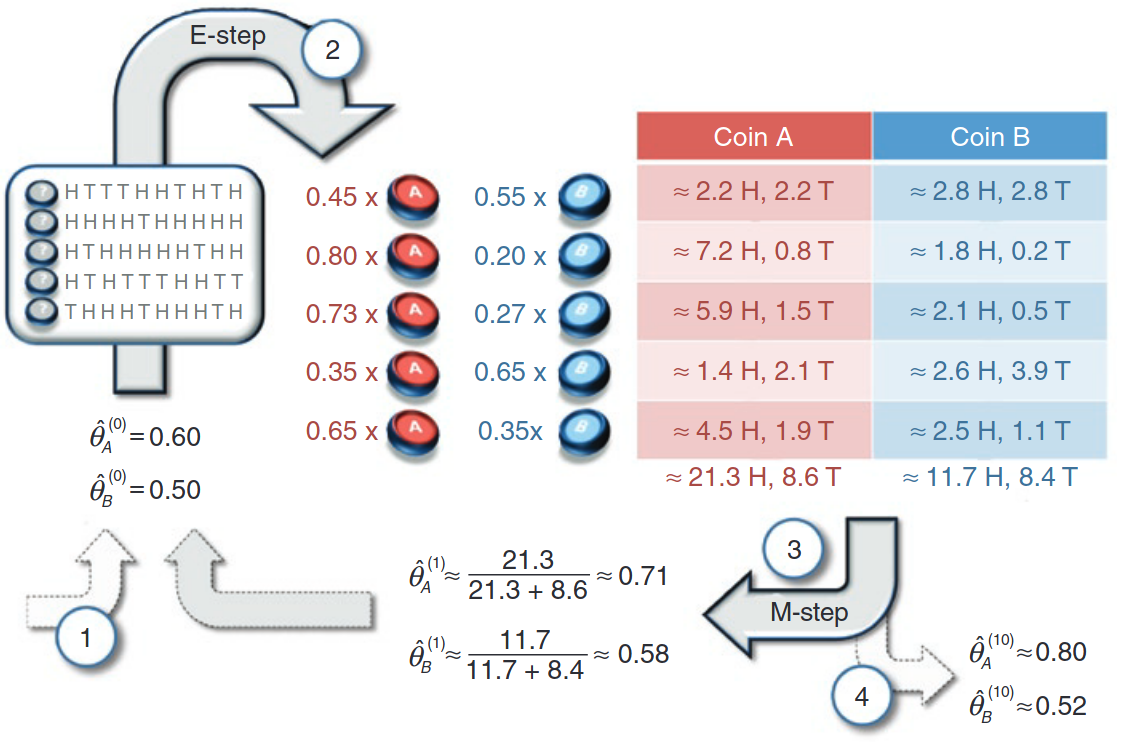
\includegraphics[width=0.7\textwidth]{chapters/BayesianNetworksLearning/mixture}
  \caption{EM algorithm step in Mixture \cite{do2008expectation}}
  \label{fig:mixture}
\end{figure}

We are know using the figure \ref{fig:mixture} to set the example in a numerical context. We are following the numbers in the diagram.
\begin{enumerate}
  \item We are considering a prior \(\bm{\theta} = (0.6, 0.5)\), a set of \(N = 5\) samples and \(M = 10\) flips per sample.
  \item This corresponds to the \textbf{E-step}, we calculate each \(Q(z_{n}\mid x_{n}, \bm{\theta})\).
    \[
    \begin{aligned}
      Q(z_{1} = A) &= \frac{0.6^{5} 0.4^{5}}{0.6^{5}0.4^{5} + 0.5^{5}0.5^{5}} \approx 0.45 \implies Q(z_{1} = B) \approx 0.55\\
      &\mathrel{\makebox[\widthof{=}]{\vdots}} \\
      Q(z_{5} = A) &\approx 0.65 \implies Q(z_{5}=B) \approx 0.35
    \end{aligned}
    \]
  \item The \textbf{M-step} corresponds to setting
    \[
    \begin{aligned}
      \theta_{A} &= \sum_{n=1}^{5}Q(z_{n})\frac{x_{n}}{10} \approx \frac{21.3}{21.3 + 8.6} \approx 0.71\\
      \theta_{B} &\approx 0.58
    \end{aligned}
    \]
  \item Step 4 represents a possible solution after \(10\) iterations.
\end{enumerate}


\section{EM Extensions}
\subsection{Partial steps}

Making a partial M-step consist on not using the optimal parameter for the energy term, but using one with just higher energy. Finding this values can be easier than finding the optimal one and convergence still follows as the only requirement to make the likelihood increase was to increase the lower bound.

On the other hand, when studying the increase on the likelihood, we supposed that the optimal E-step was being used. In general, we cannot guarantee that a partial step would increase the likelihood, even though it is guaranteed to increase the lower bound.

Another important factor is, that the EM algorithm assumes that the energy term is possible to calculate, which may not be. As an approach to solve this situation, we can set a class of distributions \(\mathcal{Q}\), and minimize the KullBack-Leibler divergence between \(P(h \mid v, \theta)\) and a distribution \(Q \in \mathcal{Q}\), so we pick a distribution such that
\[
  Q = \argmin_{Q \in \mathcal{Q}} \KL{Q(h \mid v)}{P(h\mid v, \theta)}
\]

An extreme case is to choose \(\mathcal{Q}\) as delta functions, where the energy term is now a constant. And the optimal chose setting is
\[
Q(h^{n} \mid v^{n}) = \delta (h^{n}, h^{n}_{opt}) \hspace{2cm} h^{n}_{opt} = \argmax_{h}P(h , v^{n} \mid \theta)
\]
This is called \emph{Viterbi training} and does not guarantee that the log likelihood is being increased in each iteration.
